\section{Path planning} 

Basic marine navigation is plain, because there are few distracting elements in the environment. Althpugh the maneuvering of ships is rarely restricted to open seas, without any obstacles to avoid, and even then sailing vessels require active planning, as they rarely move parallel to the wind direction, or other disturbances may apply, like ocean currents.

The problems of navigation and pathplanning will be introduced gradually. There are two kinds of boats (bowerboats and sailboats), two types of environments (still water and riverine) and two areas of applications (shortest route between points or shortest traversal of an area). In summary there are eight problems to be solved, each getting more complex than the one before. Fortunately, it's enough to solve only some key problems, then combine the findings to a roboust pathplanner.

\subsection{Model of maps and obstacles}

The forms of obstacles in the sea can vary between wide levels of complexity. The operation space can be either be completely open or closed, and they might contain very simple or very complex inner structures. Or the free space can be just a strait or as narrow as a river. In the latter case especially, the local traffic of other vehicles must never be ignored, or accidents might occur.

\begin{figure}[H]
	\centering
	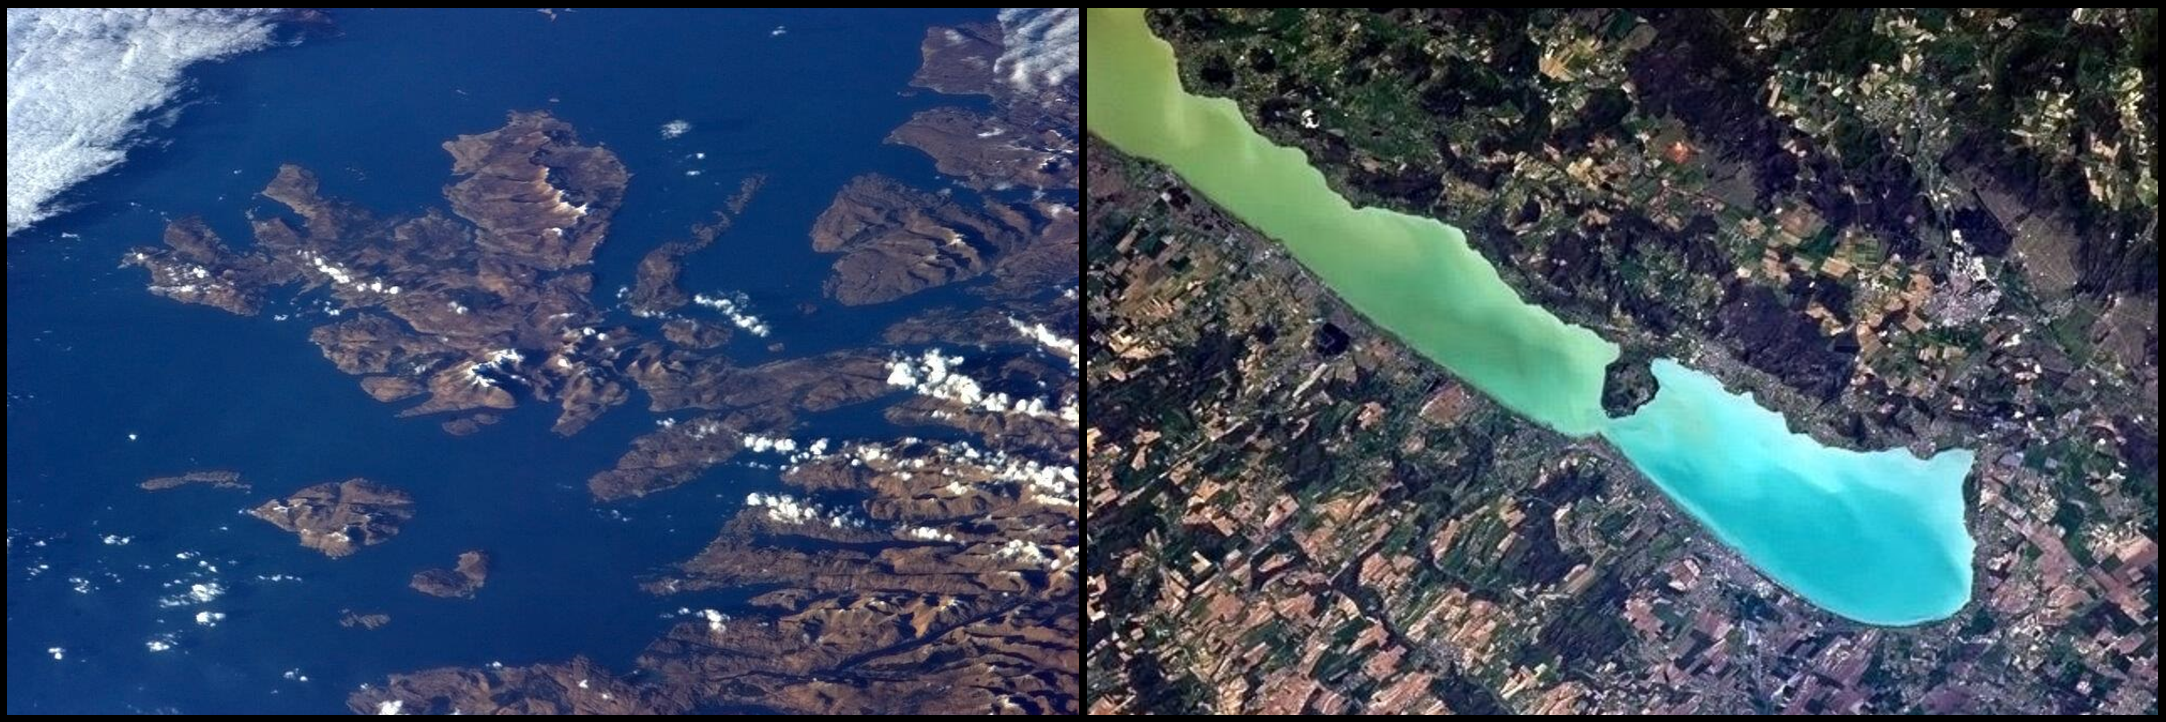
\includegraphics[width=\textwidth]{pics/hadfield}
	\caption{Isle of Skye and Lake Balaton. Photographed by Chris Hadfield}
	\label{fig:linemap}
\end{figure}

\subsection{Global Path planning}

Several algorithms have been developed for global path planning, and this field of study is still researched extensively. The different methods result in very different paths, some of them are optimal, others are not, and some algorithms might even fail to create a path at all. Their performance varies greatly by the different environments they are executed in. A complete overview of all possible motion planning strategies is not in the scope of this document. Some that might be fast, reliable and optimal in certain areas might fail completely in others. In order to find the best navigation solution for each environment, the following algorithms will be analysed and compared to each other in different settings.

\paragraph{Cell decomposition}

Cell decomposition methods are the most used and researched path planning field in outdoor robotics \cite(pathplanningoverview). The region is broken down into discrete, non-overlapping fields. the union of these fields is the original region. The method has three sub-categories, the Approximate, Adaptive and Exact Cell Decomposition. We will only discuss the Approximate method.

The most widespread of all Cell Decomposition algorithms is the A* search. It lays a grid down over the area to obtain the cell points, representing a graph. Then a best-first search is used to determine the least-cost path between the starting point and the goal. While traversing the graph, A* follows the path of lowest expected total cost. It keeps a sorted priority queue of the cells that need to be examined.

The order of the nodes to be visited are determined based on a cost function based on the past path-cost and the future-cost estimated by heuristics.

[image collage showing how A* works in different environments]

\paragraph{Roadmap}

Roadmap methods use sparse graphs to represent the connectivity between free spaces. The most commonly known algorithms in this group are the visibility graph, or Voronoi-diagram based. Although they have common basics and restrictions, they are significantly different. The former produces an optimal, but unsafe path, as it passes very close to the vertices of the obstacles, the latter generates a rather safe, but suboptimal path, because it aims to keep maximum distance from surrounding objects.

A recent approach of the problem is the Probabilistic Road Map pathplanning (PRM). It generates several random nodes around the map and checks their connectivity. The PRM results in a quick but imperfect roadmap, as it sometimes fails to detect existing connectivity or becomes inefficient, especially in case of narrow passages between vast open spaces. This problem can be solved by a different node placement strategy based on gaussian distribution distance from forbidden areas.

\paragraph{Wavefront}

The wavefront pathplanning algorithm is a simple, slow, but reliable method to determine free space connectivity, if all the above fails.

\paragraph{Comparison of algorithms}

[comparison of path length, execution time, execution efficiency (path length / execution time) in different settings]

\subsection{Local planning and collision avoidance}

\subsection{Navigation of motorboats}

The navigation of a motorboat in an open space is the most basic path planning problem. If there are no moving obstacles in sight, our only task is to keep the boat from running ashore. In order to do this, we can use a geometric pathplanning algorithm, the visibility graph search method to find the shortest euclidean path.

[image of solution]

It's important however, that turning with ships can be a costly maneuver. Therefore the cost distance between each node should be increased with an angle cost as well, as in some cases the ship must slow down to complete the maneuver.

In case of a very complex environment, or if for some reason the visibility graph algorithm can not provide a shortest route, a grid-based Wavefront algorithm is used instead. In this case it's hard to incorporate the turning penality into the algorithm, so this is an emergency-pathplanning method only.

[image of Wavefront solution]

\subsection{Navigation of sailboats}

The navigation of sailboats is much more complex, even in a static environment. The navigation problem has many solutions, and it's hard to determine which is optimal.

[]

\subsection{Navigation in moving water}

In addition to the problems that a small and crowded

\subsection{Map reading}

The main method of navigation is via GPS and known shoreline database. The ship must be outfitted with proximity sensors later, in order to ensure safe navigation through traffic. During the simulation a reference shore is being generated that simulates a typical fjordic environment: Figure~\ref{fig:linemap}. The map generator is using Random Walk Functions to generate the coastline(s).

\begin{figure}[H]
	\centering
	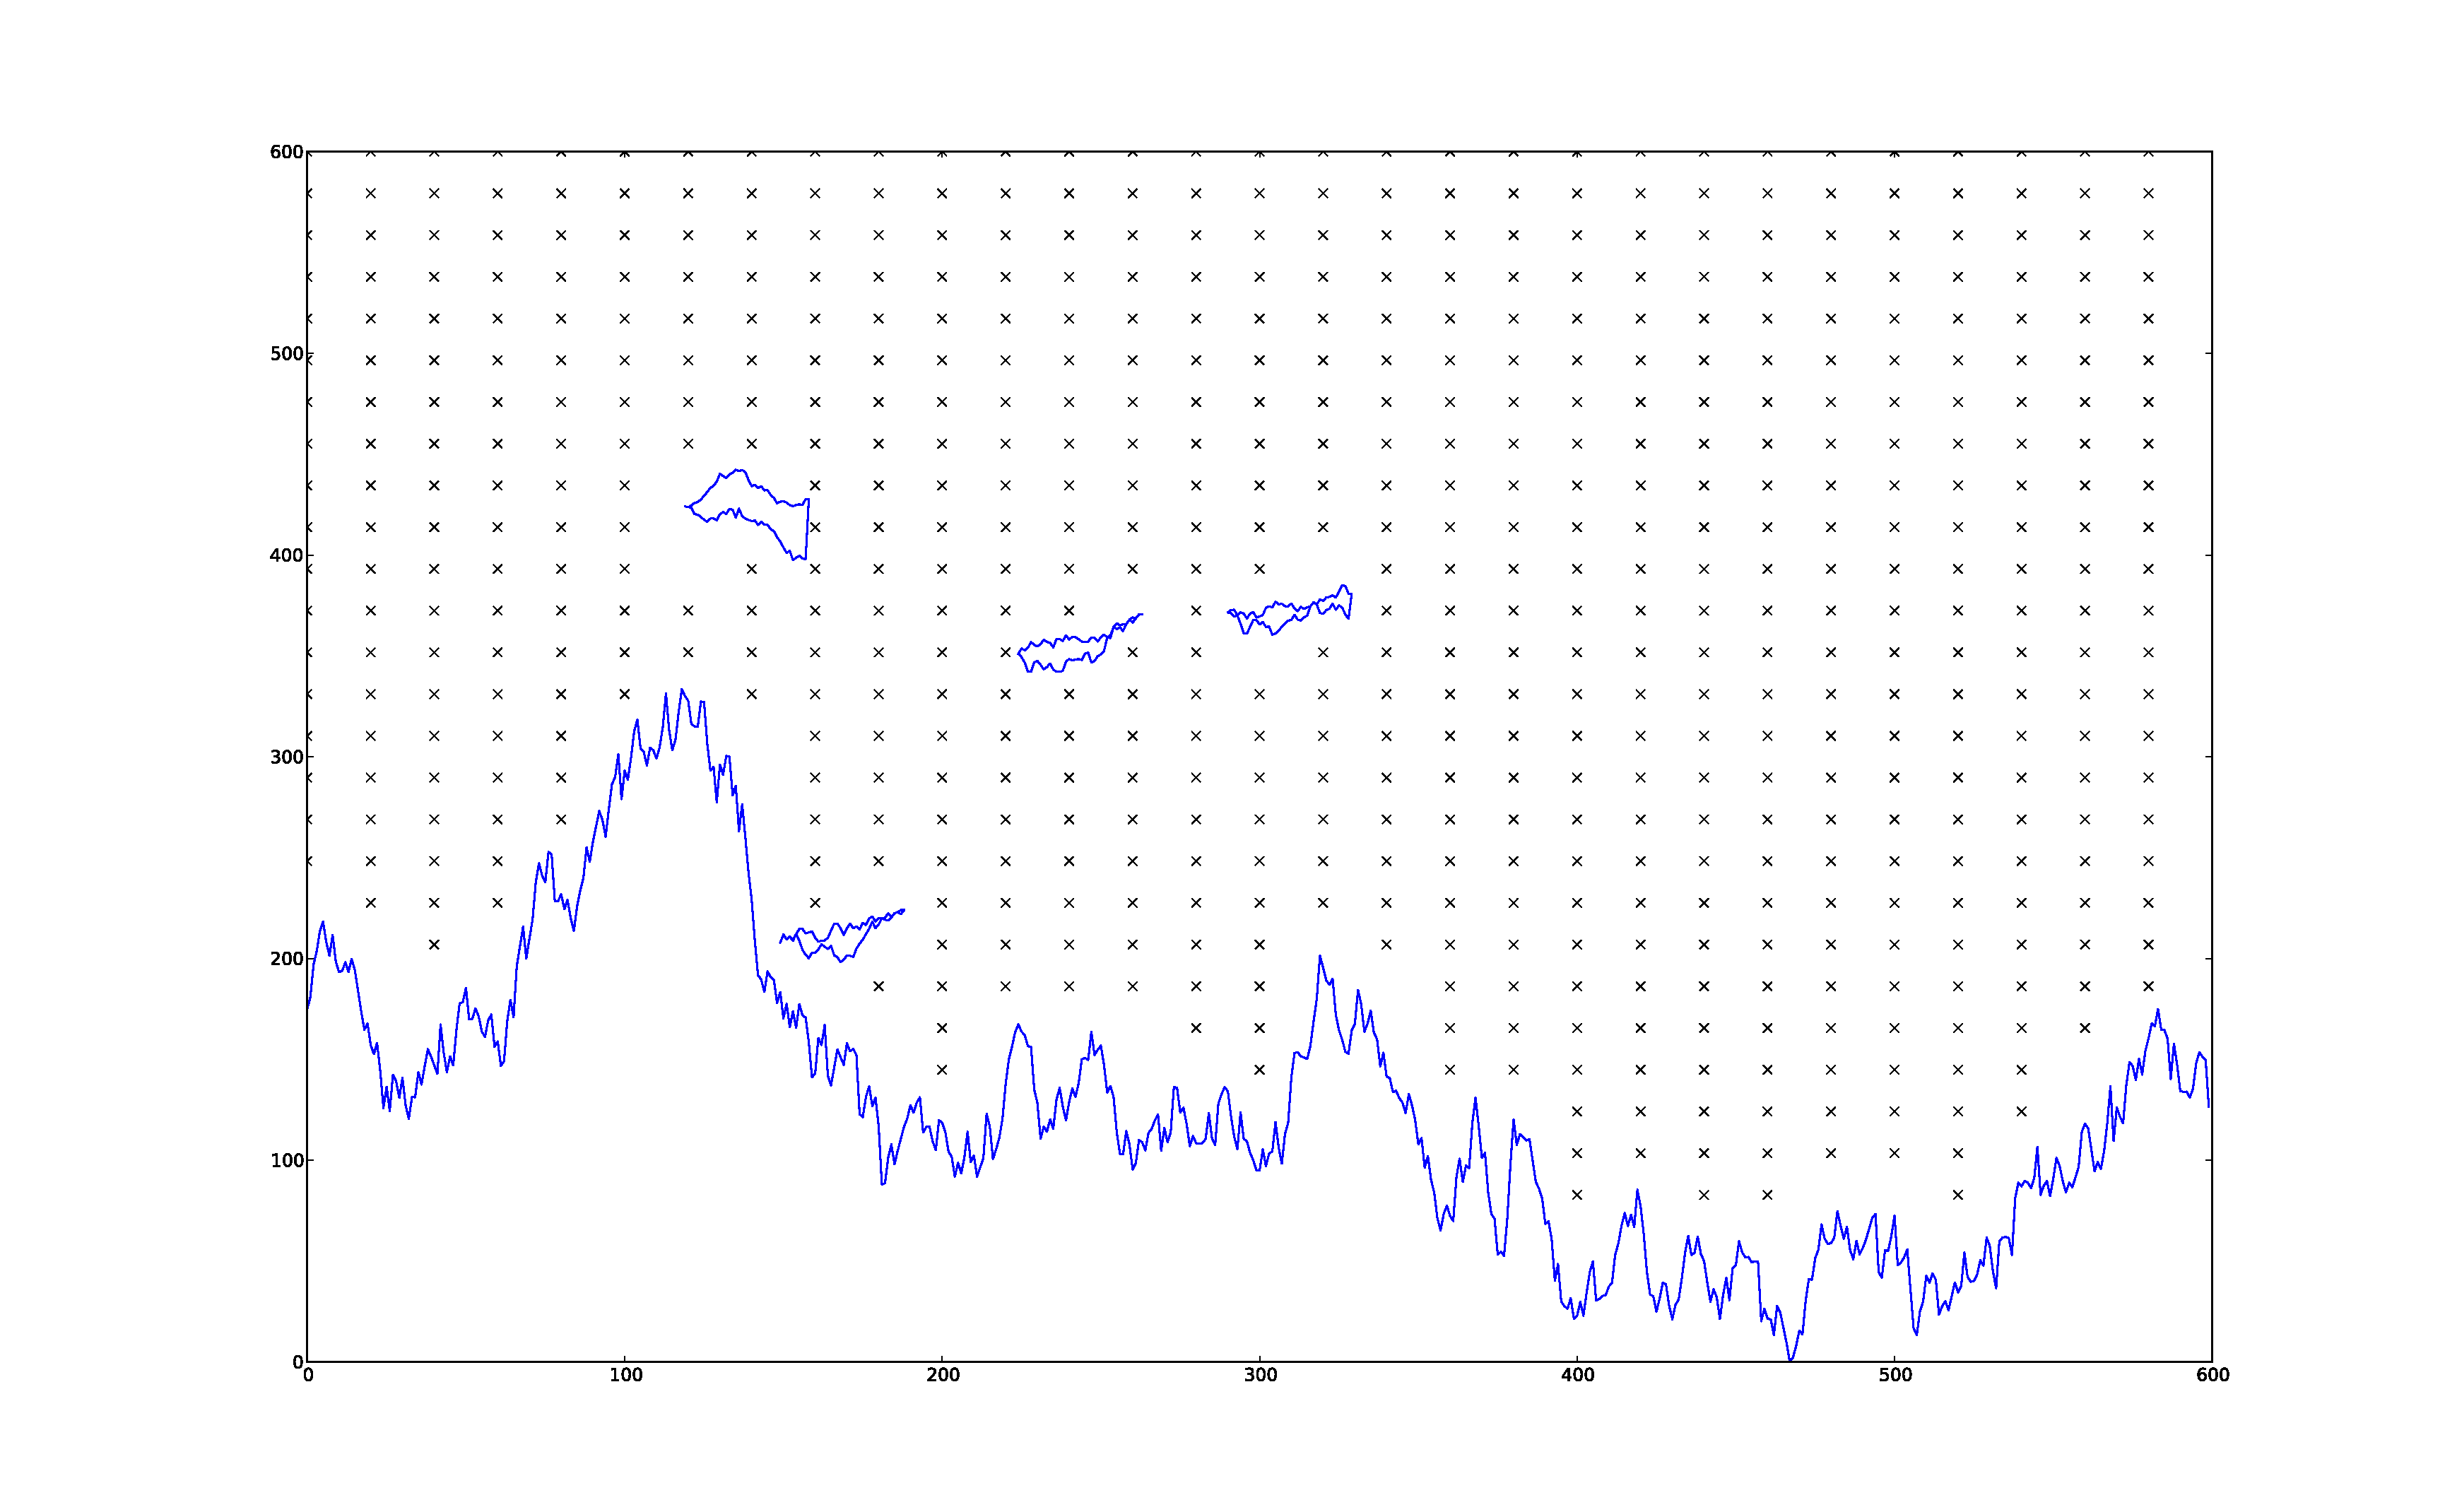
\includegraphics[width=0.8\textwidth]{img/linemap}
	\caption{The coastlines}
	\label{fig:linemap}
\end{figure}

The generated coastlines are converted to the actual Map, which is a number of surfaces: Figure~\ref{fig:solidmap}.

\begin{figure}[H]
	\centering
	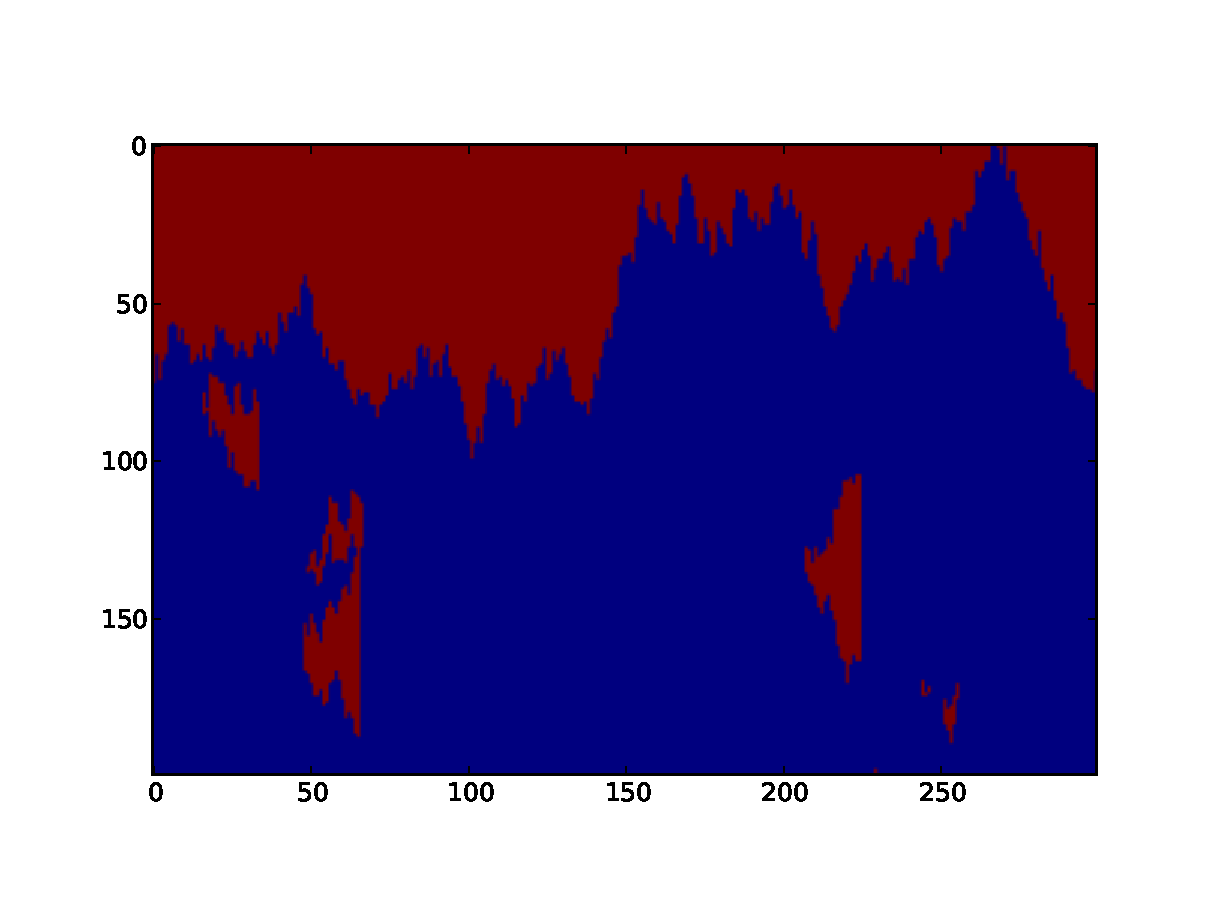
\includegraphics[width=\textwidth]{img/solidmap}
	\caption{The solidified map (the picture shows a north ("upside down") coast)}
	\label{fig:solidmap}
\end{figure}

Reading a solid map is possible from image files as well, using the Python SciPy library

\begin{figure}[H]
	\centering
	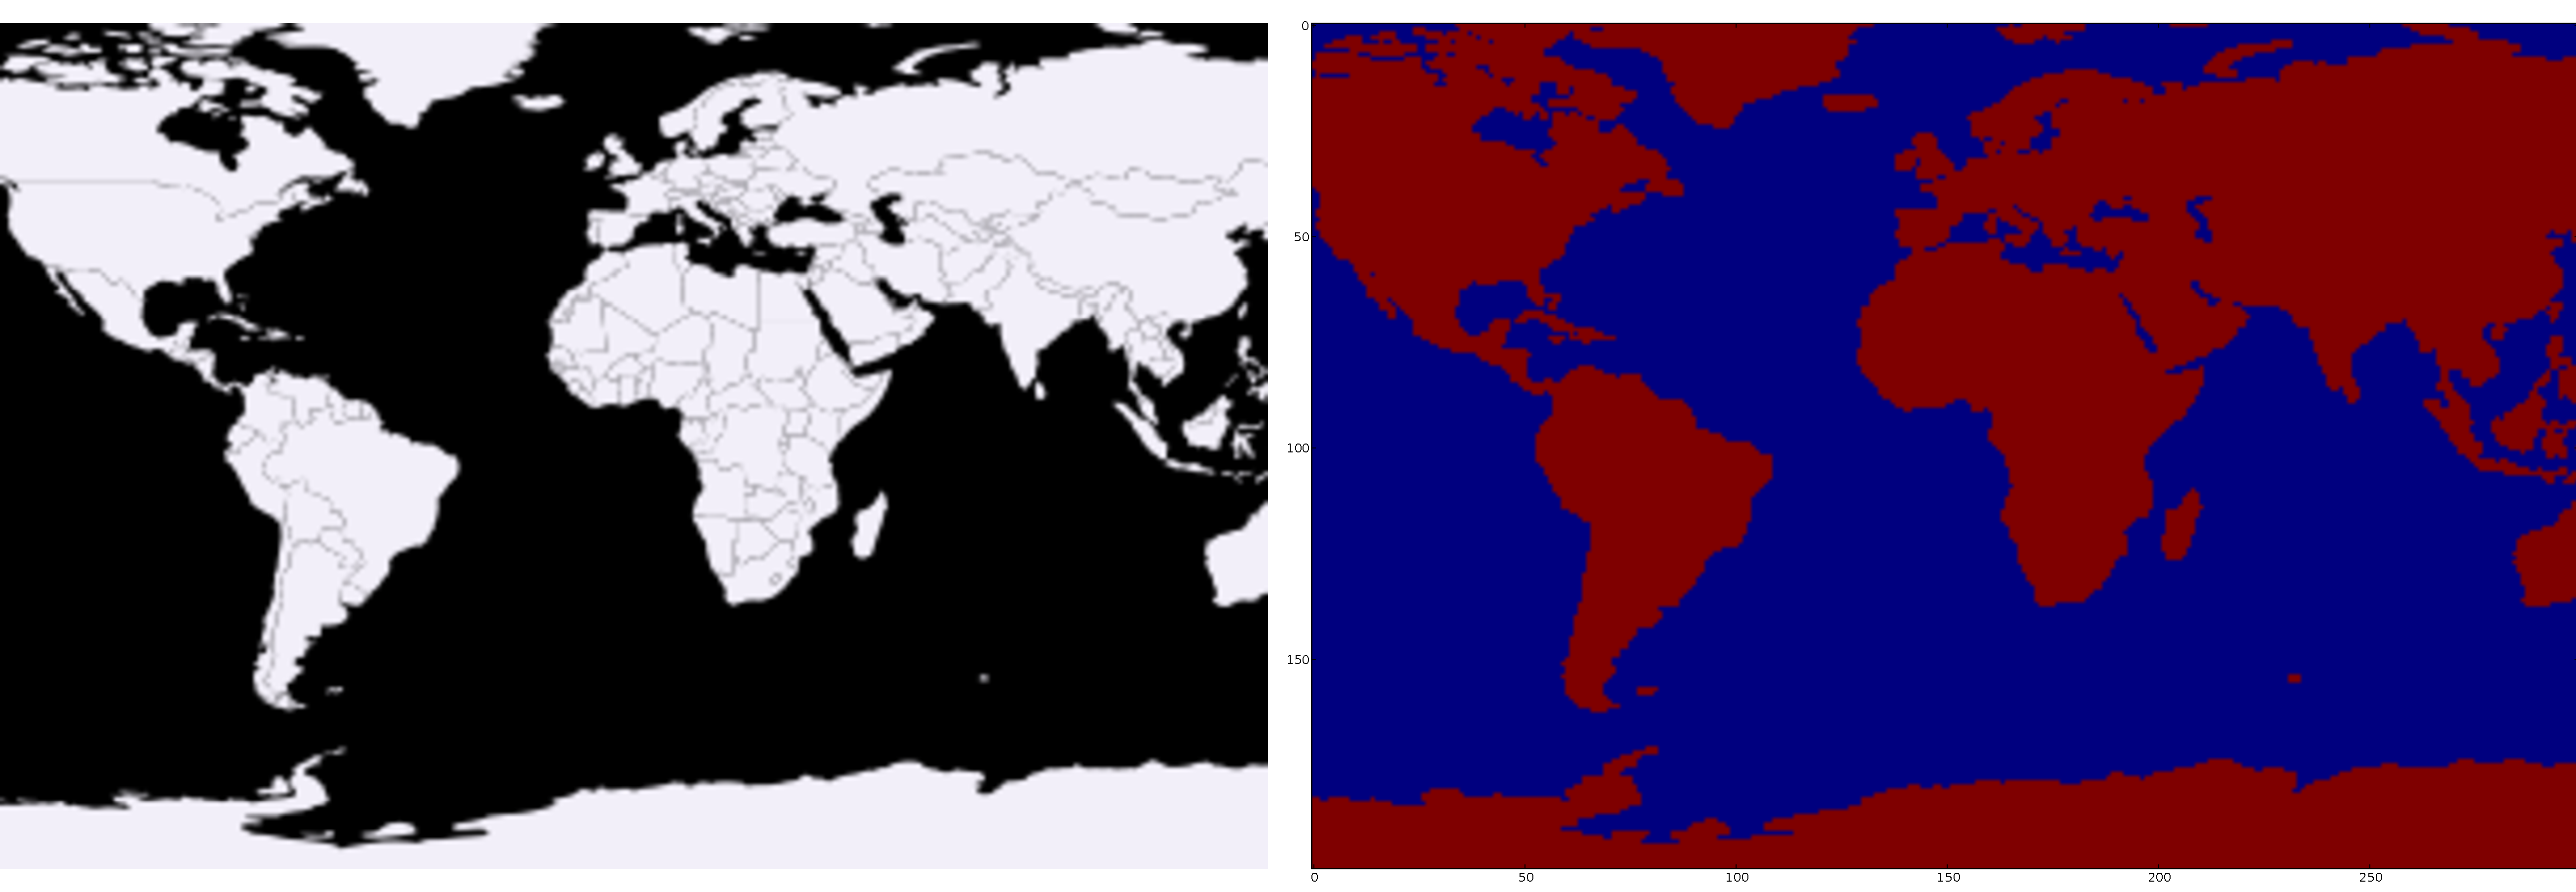
\includegraphics[width=0.8\textwidth]{img/worldmap}
	\caption{Image file processed to Map object}
	\label{fig:worldmap}
\end{figure}

\section{Routing}

Upon entering the water, the first task of the vessel in automatic or autonomus mode is to determine the course. Currently the software can not handle rivers, strong wind and magnetic declination, therefore the course is assumed to be identical to the heading.

\paragraph{The Waypoint planner} is responsible for the generating and ordering of the key measurement points. Visiting a set of waypoints on a given map leads to the Traveling Salesman NP-complete problem. Even using dynamic programming, determining the best route with the Held-Karp algorithm the program requires $O(N^2 2^2)$ steps [wiki]. The problem has been in the crosshair of mathematics for a long time, but a fast exact solution has never been found. The waypoint-planning is not time-critical, but a sufficient length of path should be calculated in a reasonable amount of time.

Fortunately the arrangement of the measurement points is relatively dense and predictable, allows only neighboring travels and repeated visits. In order to reach a suitable algorithm, some heuristics of the path planning needs to be examined.

\begin{tcolorbox}[colback=cyan!5,colframe=cyan!40!black,title=Code: Ship.py \\ https://www.dropbox.com/s/fmtsaatql7jqjhw/Ship\texttt{\_}nofilter.py]
\begin{minipage}{0,6\textwidth}
Ship.py implements the Ship Object. Everything related to the handling of a ship is encapsulated in a Ship instance. Multiple instances can be created based on the same object, with different parameters, and they are using the same resources.
\end{minipage}
\begin{minipage}{0,35\textwidth}
\raggedleft

\includegraphics[width=0.8\textwidth]{img/ship}
\end{minipage}
\end{tcolorbox}

\paragraph{In a simple coastline} the points can be placed in a certain order relative to the coast, to achieve a sufficient result. If the shore is relatively smooth, the ship can also travel parallel to the coast, to decrease the required number of turns.

\begin{figure}[H]
	\centering
	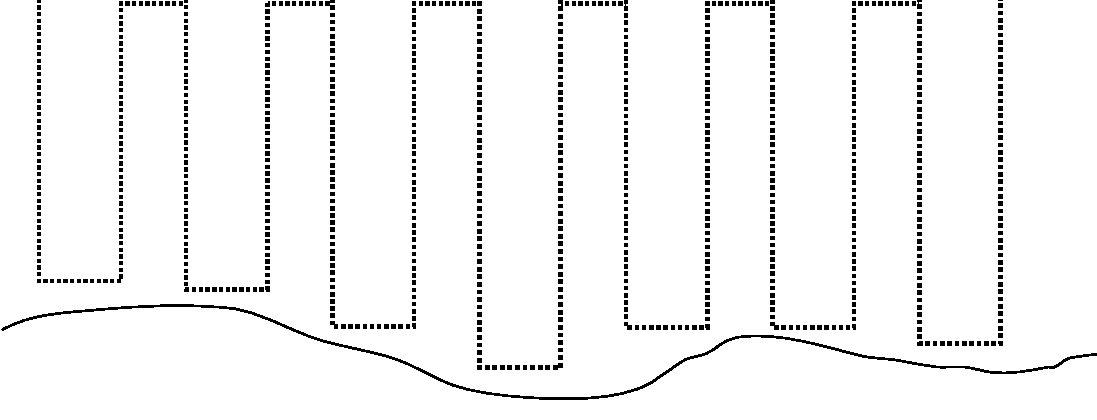
\includegraphics[width=\textwidth]{img/simplecoast}
	\caption{A simple coast and a sufficient path}
	\label{fig:simplecoast}
\end{figure}

\paragraph{Introducing isles and deep bays} to the area complicate the situation. Some waypoints need to be removed, and an avoiding path needs to be taken. This will cause many redundant measurements and very sub-optimal path, if the island density and the complexity of the coast is high.

\begin{figure}[H]
	\centering
	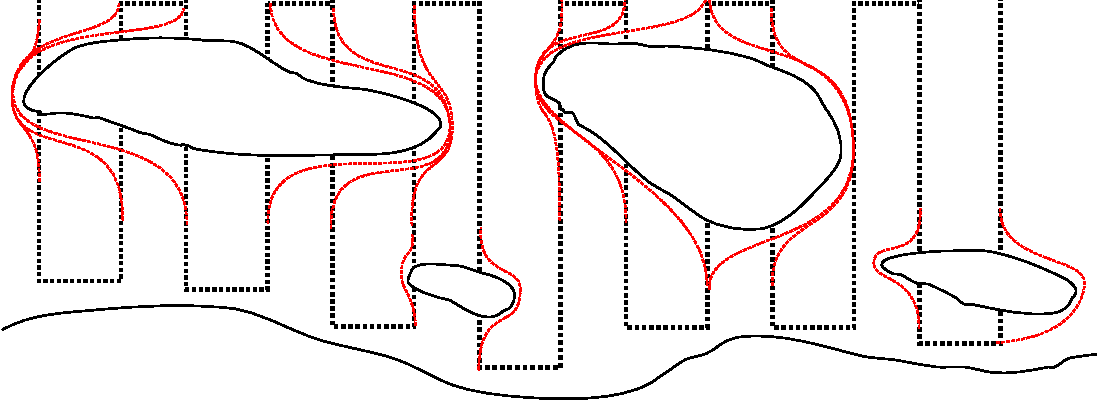
\includegraphics[width=\textwidth]{img/pathislands}
	\caption{Coast with islands}
	\label{fig:pathislands}
\end{figure}

\paragraph{Greedy traversal}

stretches a measurement grid over the area, and the points are traversed in an unpredictable way, using a neirest neighbourgh algorithm.

\begin{figure}[H]
	\centering
	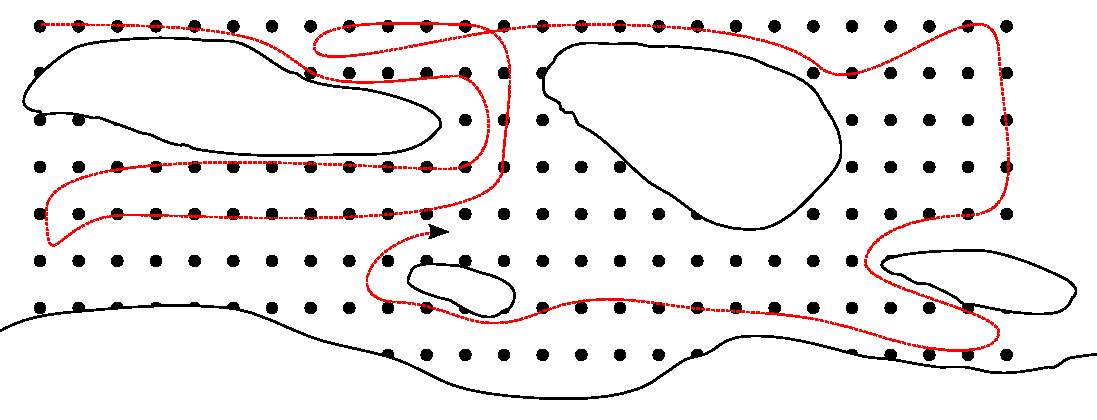
\includegraphics[width=\textwidth]{img/traversal}
	\caption{A random path based on graph traversal}
	\label{fig:traversal}
\end{figure}

 According to [citation] heuristic closest neighbour search is usually 5-10\% worse than the ideal solution. Using the closest neighbour heuristic, the simulation leads to the following path: Figure~\ref{fig:nn}.

\begin{figure}[H]
	\centering
	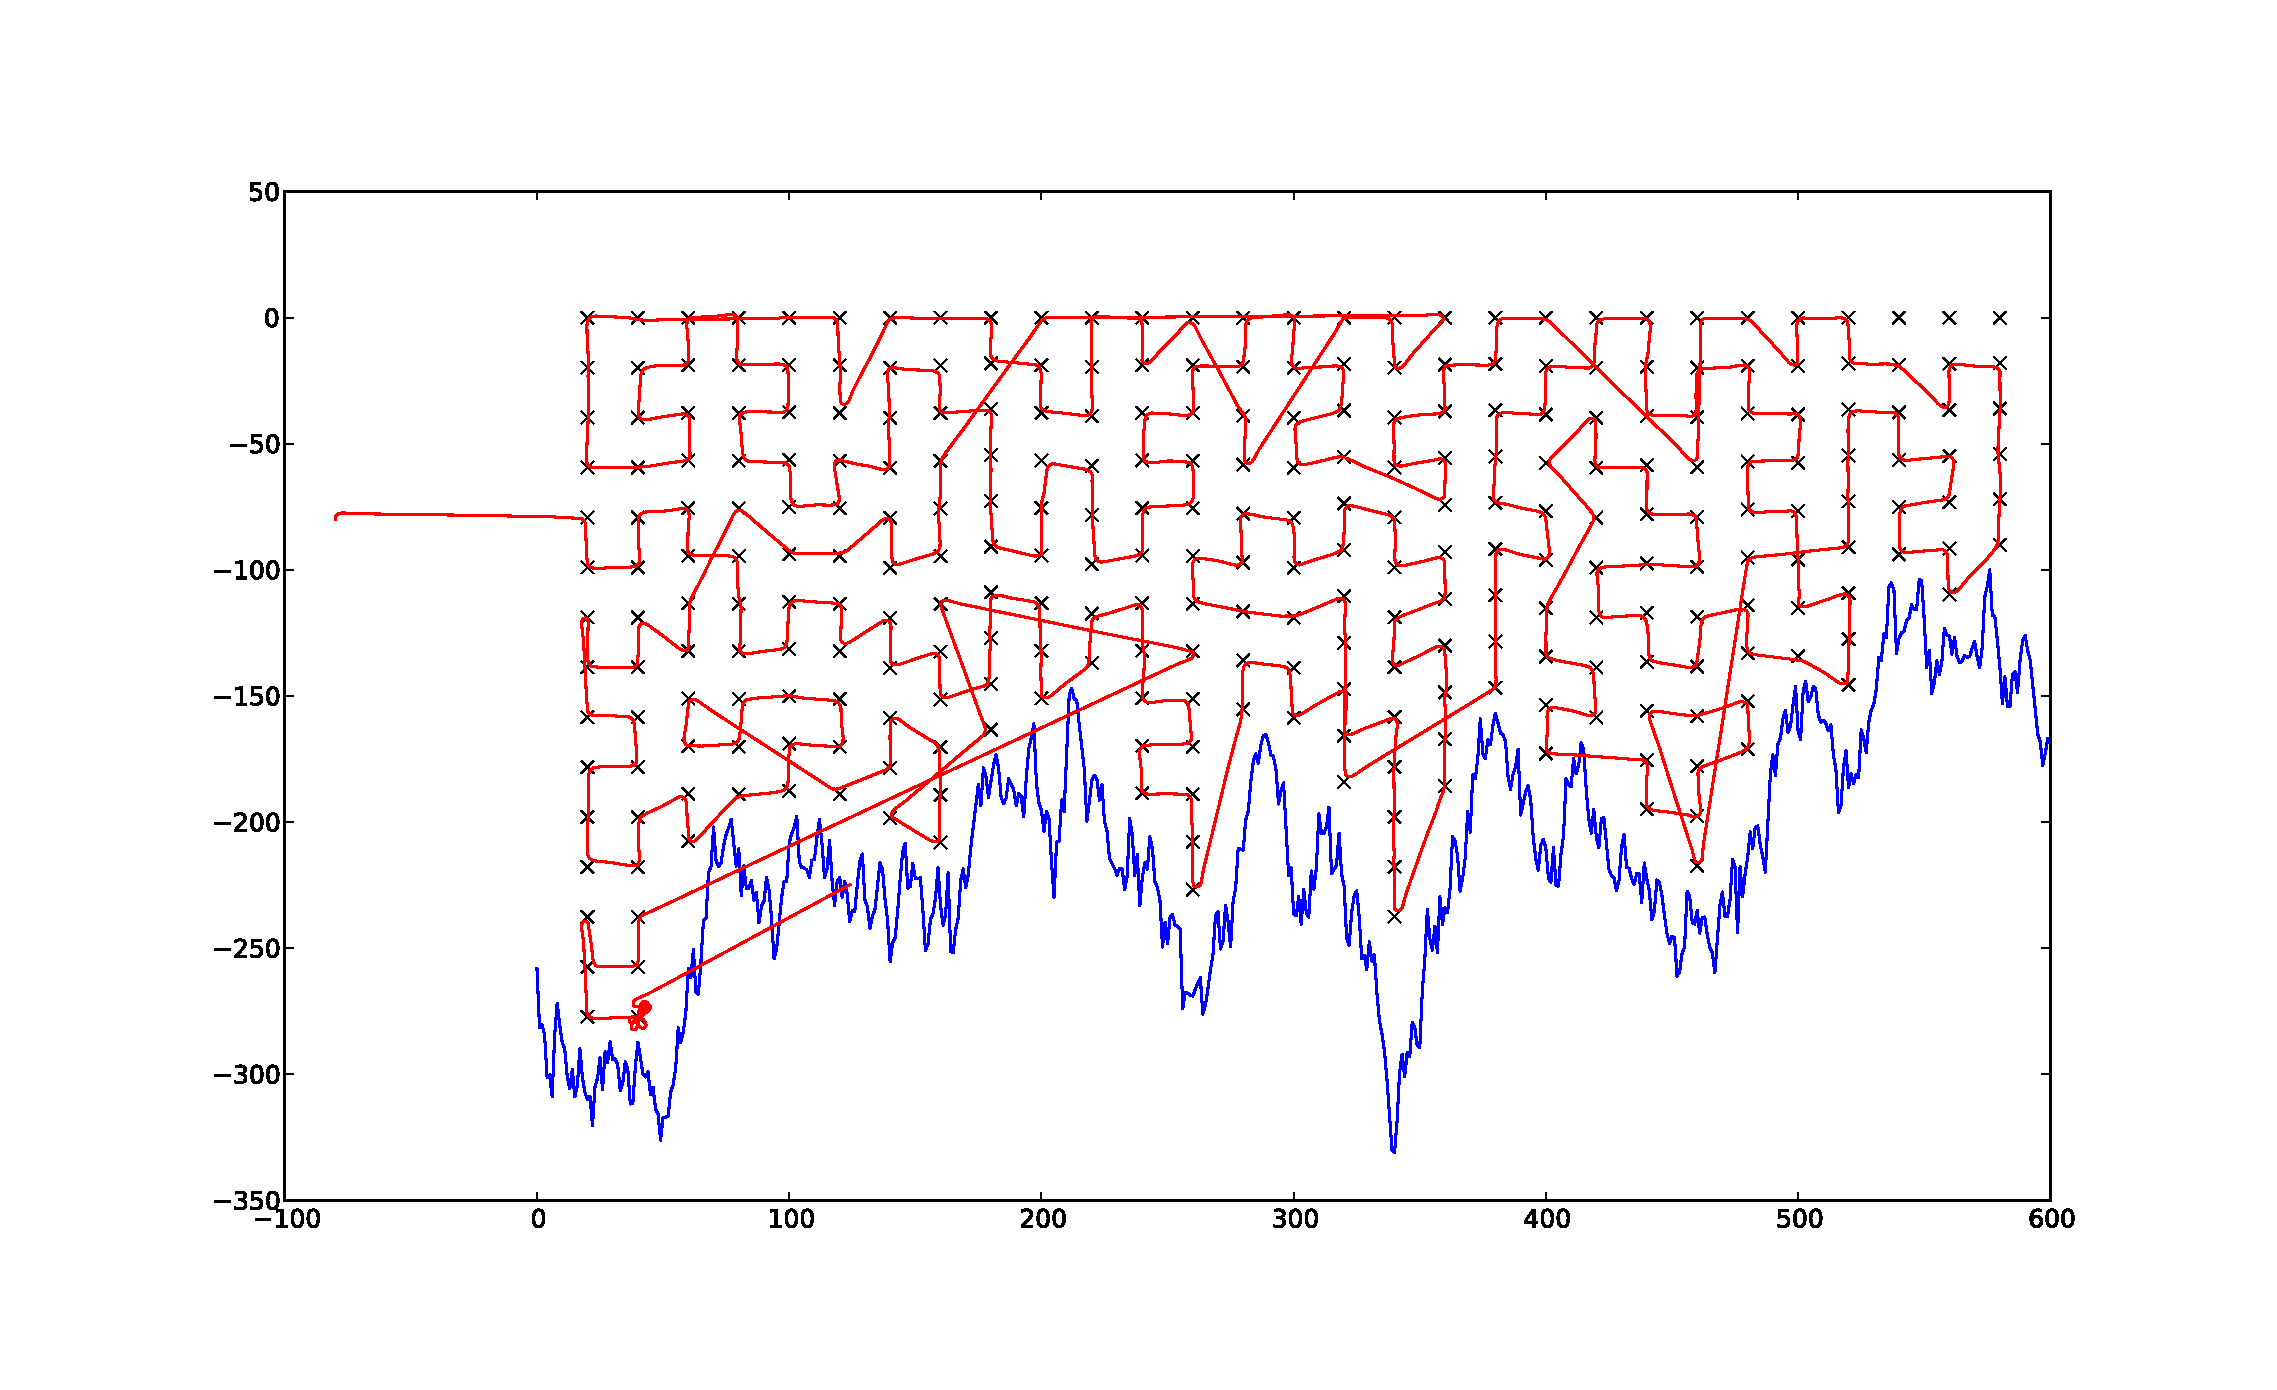
\includegraphics[width=\textwidth]{img/nn}
	\caption{Neirest neighbourgh algorithm}
	\label{fig:nn}
\end{figure}

\subsection{Lowest cost heuristics}

Even without major nautical engineering skills the following presumption can be made: If there are two paths with identical start and finish and identical lengths (start != finish) the  path with less turning is more effective.
This presumption can be extended to the following theory:

The most effective nautical path between two given points is the one with the least sum cost. The sum cost is the traveled distance times distance cost, plus absolute turnining times turning cost.

\begin{align}
	\Sigma C  = dist*C_{dist} + |turn| * C_{turn}
\end{align}

The cost of the distance and the turning depends on the type of the ship. A large, deep draught cargo ship capable of low speed will have a much higher $\frac{Distance}{Turn}$ cost ratio than a narrow military cruiser.


Using the considerations above a cost based nearest neighbour algorithm is introduced, where the lowest distance is replaced with lowest cost. The algorithm checks every point to determine which is the cheapest destination. To avoid path-loops in the map, the waypoints already visited are stored in a list. If the examined point is already in the list, the cost is increased with a redundancy value, so the algorithm will chose a different, slightly more expensive, but still unvisited measurement point. The algorithm also checks, if the path leading to the examined waypoint is clear of obsticles.

Running the simulation with the above pathplanner results in the following course: Figure~\ref{fig:lc}.

\begin{figure}[H]
	\centering
	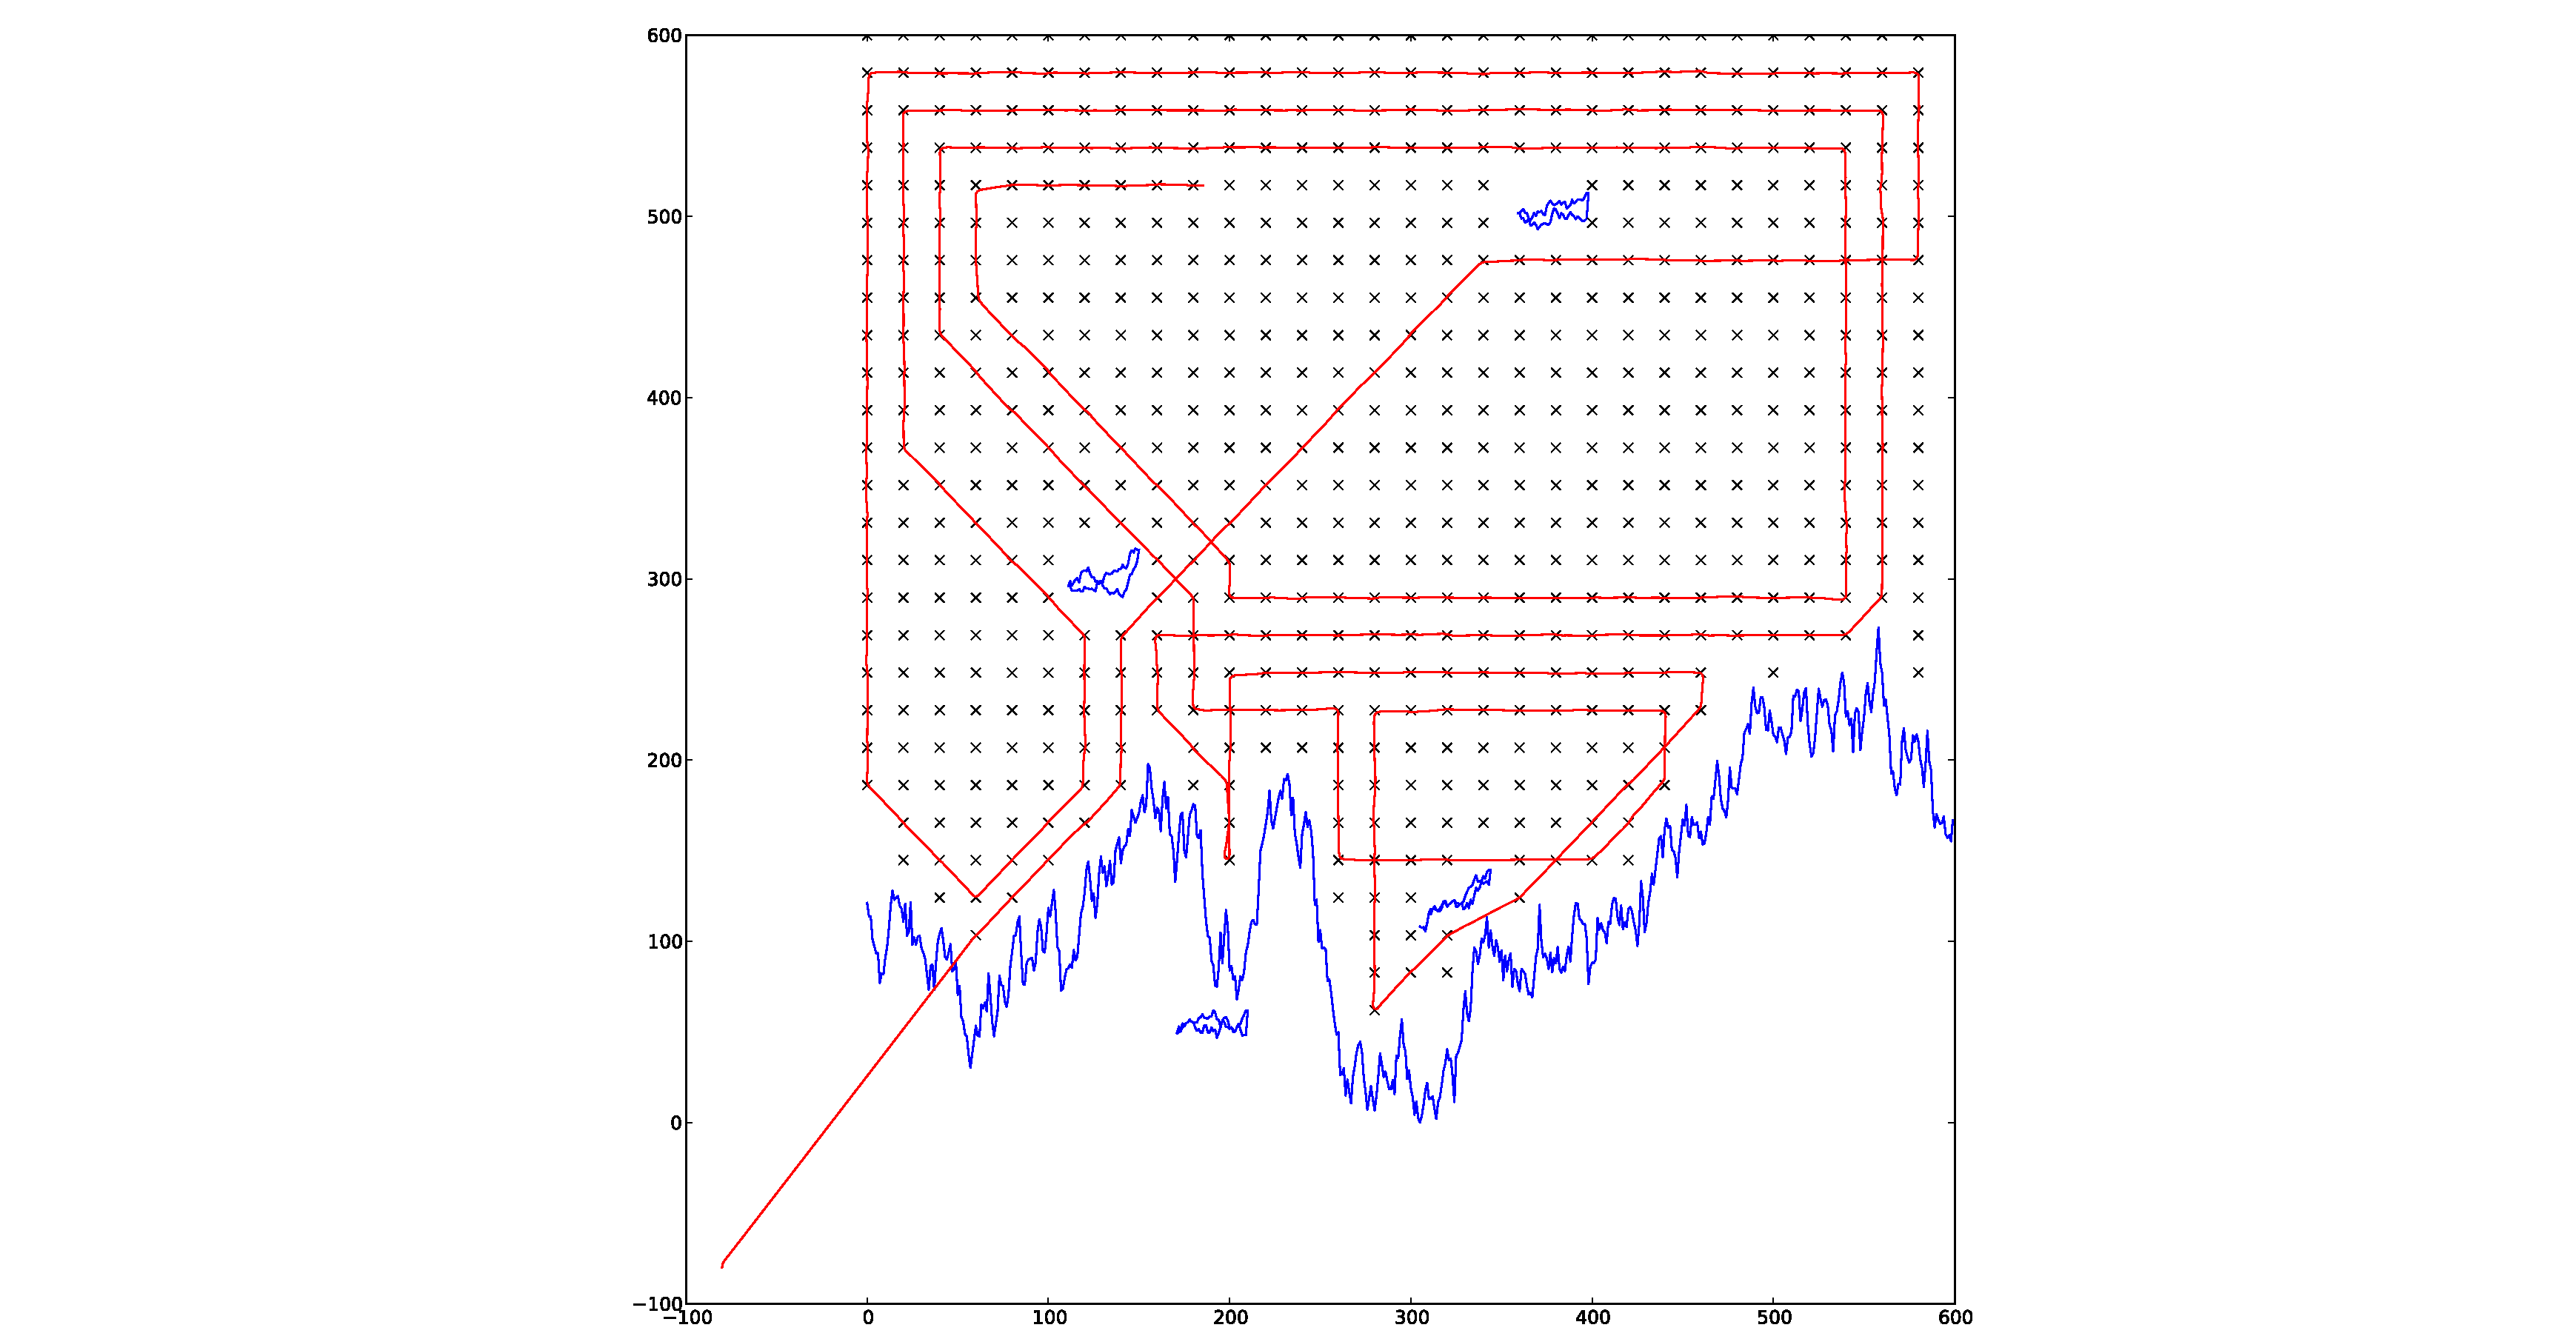
\includegraphics[width=\textwidth]{img/geee}
	\caption{Lowest cost algorithm}
	\label{fig:lc}
\end{figure}

This navigation method works adequatly in open environments. However, if the map is consisted of tight narrows and hard to navigate areas, the algorithm above fails to exit certain areas of the map. To be able to operate in such shores, a different kind of routing is required.

I call this method "Wavefront", because the points examined are moving away from the surface vessel in a circular shape (well, in a rectangular actually) like a Wavefront. The Wavefront checks every neighbouroing waypoint, that wasnt checked so far, and stores the previous life of the Wavefront. If a point is found that has not been visited before, a list of waypoints are returned, and the ship will sail through them, and reach the destination.

Figure~\ref{fig:Wavefront} illustrates this navigation method by simulating a task on the map of the Earth.

\begin{figure}[H]
	\centering
	\includegraphics[width=\textwidth]{img/Wavefront}
	\caption{Wavefront routing algorithm}
	\label{fig:Wavefront}
\end{figure}

\section{Navigation}

Once the required course has been set, the control system will take over the handling of the ship. The Navigation is the first and highest layer of control in the High Level Controller. In order to explain the navigation, the coordinate systems must be defined first.

\subsection{Frames of reference}

The operator team and the GPS sensor are using the Earth Centered Earth Fixed (ECEF) coordinate systems. Navigation on a spherical surface would introduce a lot of unnecessary calculations in every control cycle, since a plane can be fit onto the surface with minimal error, because the small vessel has limited maximum range.

During the Navigation the North East Down coordinate system is used to determine the attitude and position of the ship. The NED coordinate system is centered to the first GPS measurement coordinate.

A third Body Frame is also defined, the dynamic system of the ship was calculated in this frame.

\begin{figure}[H]
	\centering
	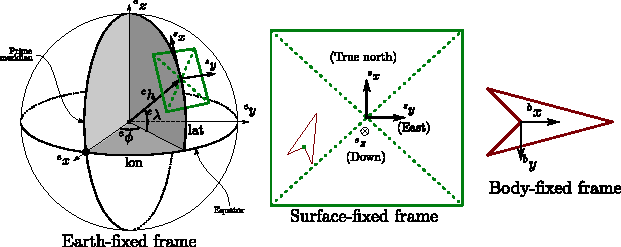
\includegraphics[width=\textwidth]{img/reference_frames}
	\caption{Used coordinate systems}
	\label{fig:coordinatesystem}
\end{figure}

\begin{align}
	\lambda = longitude  \quad \phi = latitude
	\\ GPS_{[\lambda , \phi , h]} \Longleftrightarrow [X_{NED}; Y_{NED}; Z_{NED}]
\end{align}

\subsection{Required heading}

The heading of the ship is defined in NED coordinate system. The required heading is determined by the Law of Cosines, based on the Position of the Ship and the Position of the next Sub-Waypoint.
\begin{center}
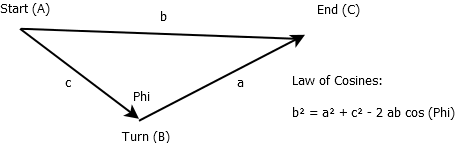
\includegraphics[scale = 0.4]{img/Law_of_Cosines}
\end{center}
Problems rise and corrections are necessary, if the heading of the ship $\theta$ is $\theta < -\pi$ or $\theta < \pi$. The heading of the ship is calculated based on the Gyro sensor and the heading can have any value in the form of: 
\begin{align}
\theta = [-{\pi} ; \pi ] \pm 2 \cdot k \cdot \pi
\end{align}\\

\begin{tcolorbox}[colback=cyan!5,colframe=cyan!40!black,title=Code: FunctionLibrary.py \\ https://www.dropbox.com/s/7nx7helisvss21a/FunctionLibrary.py]
\begin{minipage}{0,6\textwidth}
Some functions required by the software are general parametric mathematical functions, which can not be connected to any object. These functions, like the Law of Cosines, and the distance calculator function can be found in the Function Library.
\end{minipage}
\begin{minipage}{0,35\textwidth}
\raggedleft

\includegraphics[width=0.8\textwidth]{img/functionlibrary}
\end{minipage}


\end{tcolorbox}

Before invoking the control procedure, all of the heading angles must be transformed into the $[-\pi ; \pi]$ interval.
This procedure causes a possible error though.

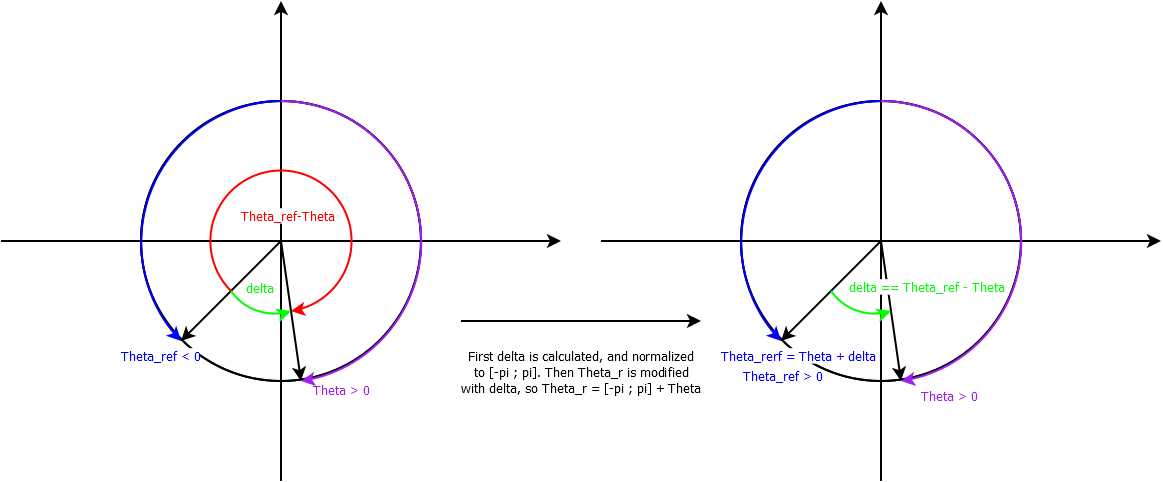
\includegraphics[width=\textwidth]{img/Headings}

The required heading or the heading of the ship must be transformed into a different representation, where 
\begin{align}
|\theta_{r}-\theta| < \pi
\end{align}
To keep a consistent heading representation, first the deviation angle 
\begin{align}
\theta = \pi_{r}-\pi
\end{align} is calculated, than transformed to the $[-\pi;\pi]$ interval and finally, with $\delta$ we can transform $\theta_{r}$ to 
\begin{align}
\theta_{r}(\theta) = \theta + \delta
\end{align}
If the conditions above are met, $\theta$ and $\theta_r(\theta)$ will always yield values that result in correct controller output.

\subsection{Waypoint planning}

\subsection{Waypoint ordering}

\subsection{Comparsion of methods (length/WP)}

\subsection{Map reading}